\documentclass[12pt,letterpaper]{article}

\title{
\textbf{\LARGE OBD Bluetooth Interface and Android App} \\
\Large Interim Technical Report Document
}

\author{
\normalsize Patrick Landis (pal25) \\
\normalsize Schuyler Thompson (sdt16) (Current Team Lead) \\
\normalsize Advisor: Swarup Bhunia, PhD
}
	
\date{\normalsize March 4, 2013}
\usepackage[margin=1in]{geometry}
\usepackage{graphicx}
\usepackage{epstopdf}
\usepackage{pgfgantt}
\usepackage{indentfirst}
\usepackage{float}

\begin{document}

\maketitle
\newpage

\section*{Executive Summary}
A user with an Android based phone will be able to read and interpret diagnostic and operational data from their 1996 model year or newer car. On some models, they will be able to control some aspects of the car, such as starting the engine or rolling down the windows. This will be accomplished by having their Android device pair with a OBD (On-board Diagnostic) interface that is connected to the car over bluetooth, using a secure channel. 

\newpage

\section{Introduction}
\subsection{General Information}
Every car in the United States since 1996 is required, by law, to contain on-board diagnostics. This standard, codified in SAE J1939 as on-board diagnostics II (OBD-II). The OBD-II specification officially requires a few different things. The OBD-II specification requires that all cars make available data link connector and also place restrictions on where they can be placed. The specification defines a set of standard diagnostic trouble codes, the freeze frame (which is sort of like a black box from an airplane, in that it records when something goes wrong), and requirements for MIL lighting (which deals with the check engine light). In addition it also defines specific terminology and acceptable limits for emissions controls components. A device is then plugged into the data link port to read messages over various protocols implemented by the car manufacturer. \\

Currently, technicians must manually plug in a device into this port in order to read OBD-II messages. Furthermore the current solutions only have basic functionality and are primarily for technicians. Our project aims to add wireless functionality for OBD-II via Bluetooth to be interfaced with Android compatible devices. Furthermore this project aims to make communication cryptographically secure. By allowing for cryptographically secure wireless OBD-II messages to be transferred to fairly ubiquitous Android-enabled devices this project is geared to enthusiasts and curious electronic hackers. \\

There are numerous design problems being tackled here. One of the primary ones is the interfacing with all of the different protocols OBD-II supports. These each have very different electrical chararataristics, and need a separate circuit designed for each one of them. Another problem is keeping the power consuption low so the whole system can be powered off of a car's battery. This also presents the problem of dealing with a non-reliable power source. Car batteries' voltage is notoriously non-stable. The system needs to be able to deal with this problem and provide stable 5V and 3.3V rails. \\

Another problem is interfacing the purposed device with all five of the OBD-II supported protocols. Not only do all of these protocols need to be supporedt but the device must figure out which protocol a car is using to communicate, the problem is further complicated with the fact that some of the protocols have the same physical layer which others share the same data-link layer of the communication stack. 

\subsection{The Five Protocols}
\subsubsection{SAE J1850 VPW}
The J1850 VPW is a communication protocol used by GM cars between 1996 and 2008. It is a variable pulse width protocol which runs at 10.4 kbps. Since the protocol is used on a bus it uses carrier sense multiple access and non-destructive arbitration (CSMA/NDA) to decide who communicates along the bus. Essentially what happens is that the if two signals ever compete for time on the communication bus the signal with the highest priority will win. It should be notec that the J1850 VPW and J1850 PWM protocls share the same data-link layer even though their physical layers are quite different. The message length is restricted to 11 bits, including its cyclical-redundancy check (CRC).
 
\subsubsection{SAE J1850 PWM}
The J1850 PWM communication protocol, primarily used in Ford vehicles, is a pulse width modulated signal. The protocols specified frequency is 41.6 kbps and use the same bit arbitration scheme above when collisions on the bus occur, CSMA/NDA. It should be notec that the J1850 VPW and J1850 PWM protocls share the same data-link layer even though their physical layers are quite different.

\subsubsection{ISO 9141-2 LIN and ISO 14230 Keyword Protocol 2000}
The ISO 9141-2 protocol is implemented as a local interconnect network (LIN). It operates at a bit rate of 10.4 kbaud. Data collisions are taken care of by the transceivers in the network. It is a digital protocol meaning that messages are encoded simply as high or low voltages. ISO 9141-2 shares the same physical layer as ISO 14230.

\subsubsection{ISO 15765 CAN}
The ISO 15765 specifies the physical and data-link layer for a controller area network (CAN). The protocol operates on a range of bit rates from 250 kbps to 1 Mbps. Bit arbitration is taken care of by CSMA/NDA and messages are passed along a bus to nodes in the network. By 2008 all light weight vehicles sold in the US must implement the CAN protocol. There are two types of data-link layers for the CAN protocol, regular and extended.

\section{Project Specifications}
This project has quite a few objectives because there are quite a few parts to it. This section will refer to Appendix I, a diagram which shows the information exchange, to clarify things.

\subsection{OBD-II Interface Component}
\begin{itemize}
	\item This component requires a circuit which will have the functionality to interface directly to a car's OBD-II port. 
	\item This component is required to plug into the data link connector specified in the OBD-II specification SAE J1962
	\item This component will need to be able to act as a transceiver with the OBD-II port.
	\item The component will also be responsible for encoding and decoding messages for each of the protocols allowed in the OBD-II standard which are:
	\begin{enumerate}
		\item SAE J1850 (VPW)
		\item SAE J1850 (PWM)
		\item ISO 9141-2  (LIN)
		\item ISO 14230 (Keyword Protocol 2000)
		\item ISO 15765 (CAN)
	\end{enumerate}
	\item This component will be required to communicate with the central microcontroller in via UART.
	\item This component will be powered from the OBD-II port.
	\item This component will be responsible for buffering messages until they can be sent to the MCU.
\end{itemize}

\subsection{Bluetooth Interface Component}
\begin{itemize}
	\item This component will be required to adhere to the Bluetooth 2.1+ specification.
	\item This component will be required to communicate with the central microcontroller in via UART.
	\item This board will be responsible for communicating via Bluetooth to Android enabled devices.
	\item This component will be powered from the OBD-II port.
	\item This component will be responsible for setting up Bluetooth communications with Android enabled devices.
	\item This component will be responsible for negotiating the shared key for cryptography purposes.
\end{itemize}

\subsection{Central Microcontroller}
\begin{itemize}
	\item This MCU must be able to communicate with the OBD-II interface component via UART.
	\item This MCU must be able to communicate with the Bluetooth interface component via UART.
	\item This component will be powered from the OBD-II port.
	\item MCU will be used to control message flow of the system.
	\item The MCU with be required to store a list of recent pairing keys to allow Android devices to auto-connect.
\end{itemize} 

\subsection{Bluetooth Functionality Android-side}
\begin{itemize}
	\item There will be writing an Android app to receive data from the OBD reader.
	\item It will use the Android SDK to implement the bluetooth functionality.
	\item The app will be able to display all of the basic messages from the diagnostic part of OBD.
	\item This includes the fault codes, monitor readiness, and whether the malfunction indicator light (MIL) is on or off.
	\item The OBD fault codes follow a pattern of N0000, a letter followed by 4 numbers. The app will contain the database of all of the standard codes and their meanings for easy lookup. 
	\item  The monitor readiness is indicating whether the all of the monitors used by the OBD system are ready to make a reading. They are reset when the OBD system is reset, and if the monitors are set to not ready, the car will fail any emissions check performed by a DMV. 
	\item The MIL is the light commonly known as the check engine light. 
	\item The app will use the Android Holo theme, and will follow the generally accepted design principals of Android UI design.
	\item The app will pair with one dongle at a time.
	\item The app will work with Android 4.1.

\end{itemize}

\subsection{Cryptographically Securing Messages}
This section doesn't describe any specific component of the system. This section describes functional requirements for the overall system to cryptographically secure wireless messages. The basis of this approach is to use Bluetooth's Secure Simple Pairing for security. This pairing protocol is mandatory for all BT 2.1+ devices.

\begin{itemize}
	\item Will use ``Just Works" form of pairing.
	\item The pairing key will be stored on the non-Android side of communication in the MCU.
	\item Both devices must acknowledge the pairing request.
\end{itemize}

\section{Methodology}
\subsection{Introduction}
The group is using a variety of design principles to accomplish this design that happen in stages. The first stage of the design was the research portion of the project. This amounted to essentially reading up on OBD-II standards as well as Android development documentation. Some research effort was also put into looking up the market outlook for such a product. After the research phase was the design phase. In this phase of the project the hardware was designed and the Android applications functionality was outlined. Both of these portions were designed to the specifications listed above in section 2 of this document. \\

\subsubsection{Hardware}
In terms of hardware the design was largely constrained to fit to the OBD-II specification, where freedom was available parts were choosen based off three main criteria: price, safety margin, and ease of use. First and foremost the device must be safe to use as a general rule parts that were choosen to work in critical areas (such as the voltage regulators) with a safety margin of 2x meaning that if a requirement was rated at a value of y a part was choosen with a rated value of twice as much or 2y. Secondly parts were choosen that were easy with which to design. This means that where applicable transistors were choosen over MOSFETS, and discrete components were choosen over IC's. This also has the added benefit of keeping the costs low. Finally in an additional measure the specs were somewhat designed based on the circuits labs' inventory since for every component available in the lab means that the lead time and price associated with buying such a part are effectively zero. 

\subsubsection{Software}
The software will be using the standard ELM327 OBD software protocol. This is a well supported serial protocol for communicating with OBD transceivers. This will allow the Android app to communicate with other ELM327 based OBD trancevers. The protocol serialization and deserialization is also well isolated in order to let us swap out a different command set if needed in the future without affecting the rest of the app. 


The app is also using the standard Android built-in themes so it will be visually appealing. This makes it both easier to develop and potentially have higher sales because of the professional look. 

Finally, the app will only be using the bluetooth radio when needed, because using the radio uses a lot of battery on the phone. A big selling point on Android is making sure your app does not hold wakelocks that keep the phone's CPU in a high power state when not needed, because Android doesn't aggressively kill apps that use too much CPU.

\subsection{Chosen Design}
\begin{figure}[H]
\centering
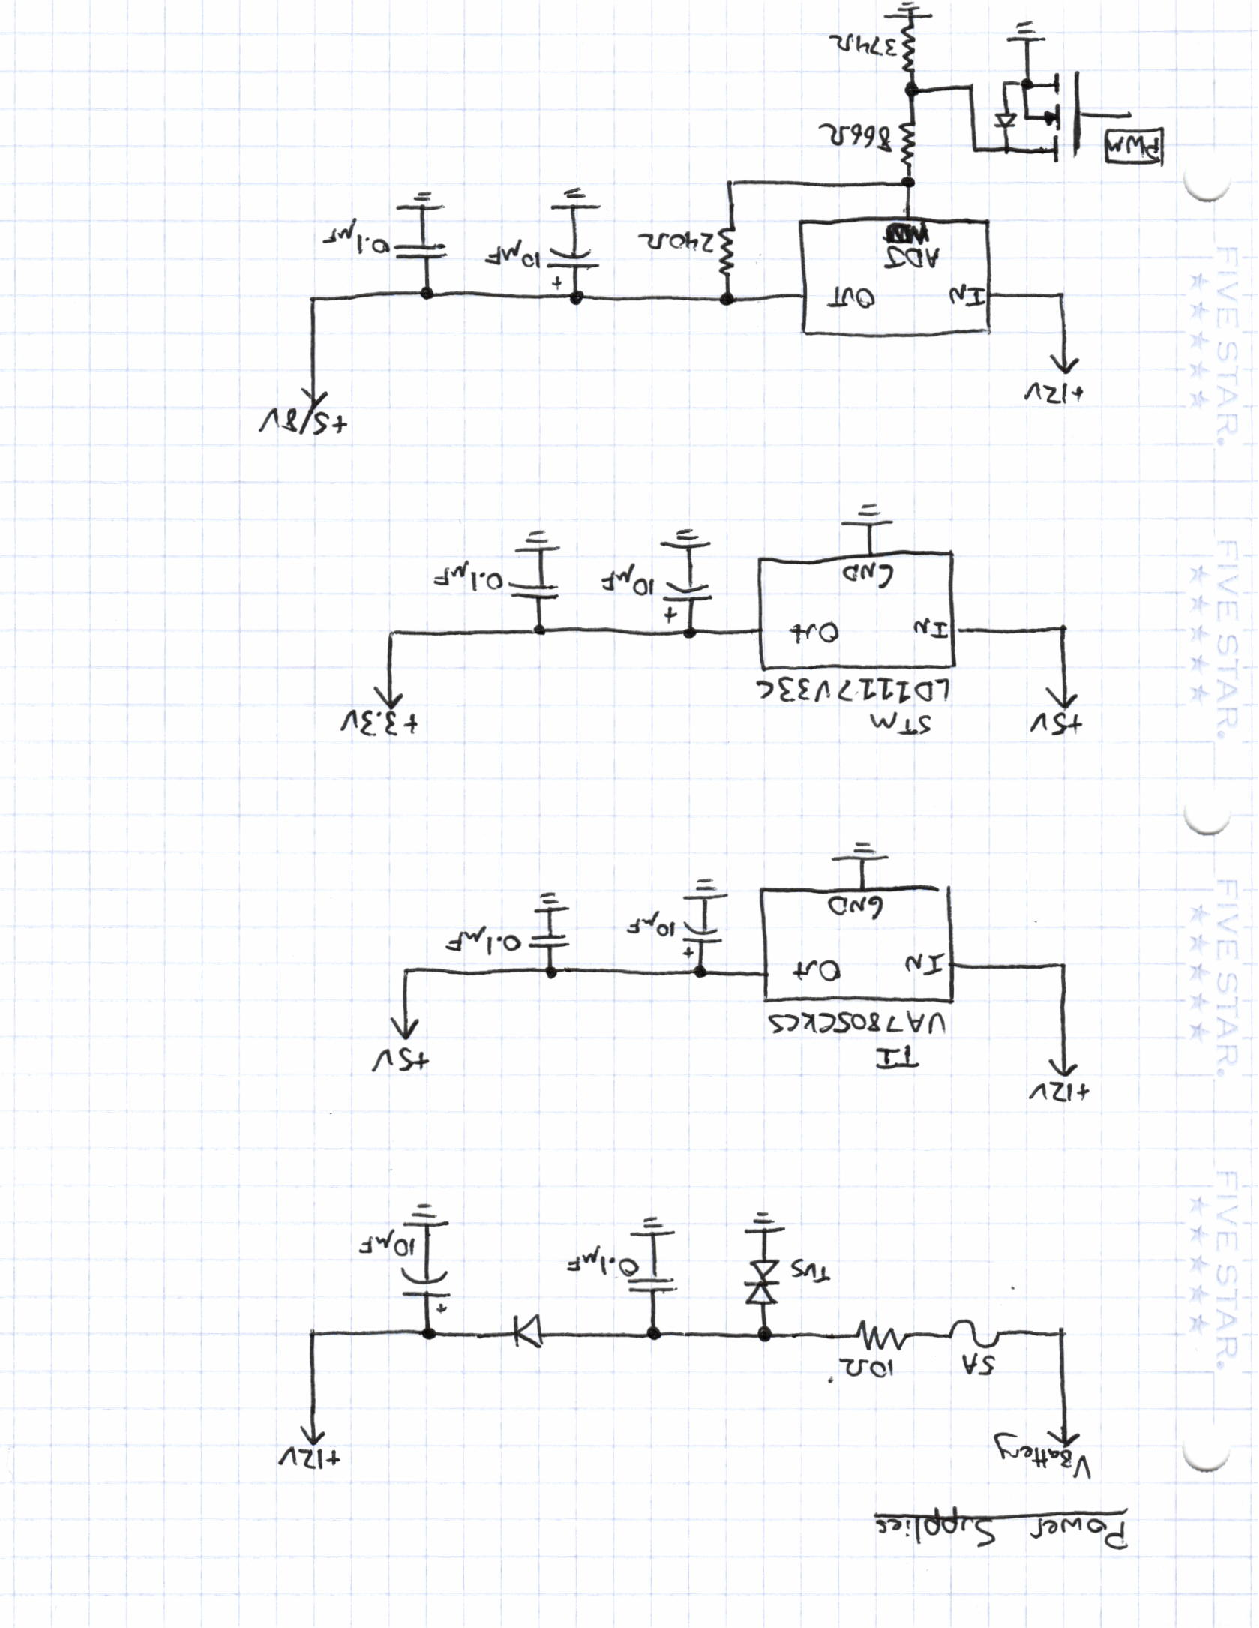
\includegraphics[page=1, totalheight=20cm, angle=180]{images/circuit_sch.pdf}
\caption{Circuit Schematics}
\label{fig: image}
\end{figure}

\begin{figure}[H]
\centering
\includegraphics[page=2, totalheight=20cm, angle=180]{images/circuit_sch.pdf}
\caption{Circuit Schematics}
\label{fig: image}
\end{figure}

\begin{figure}[H]
\centering
\includegraphics[page=3, totalheight=20cm, angle=180]{images/circuit_sch.pdf}
\caption{Circuit Schematics}
\label{fig: image}
\end{figure}

\begin{figure}[H]
\centering
\includegraphics[page=4, totalheight=20cm, angle=180]{images/circuit_sch.pdf}
\caption{Circuit Schematics}
\label{fig: image}
\end{figure}

\begin{figure}[H]
\centering
\includegraphics[totalheight=15cm]{images/info_exchange_diagram.eps}
\caption{Information Flow Diagram}
\label{fig: flow}
\end{figure}

Figure \ref{fig: flow} shows the information flow from the bluetooth module to the Android phone. The data is encrypted before it is sent over the air. This also has the effect of not allowing random devices to connect to the bluetooth module. 

\subsection{Alternative Designs}
\subsubsection{Hardware}
In terms of hardware a few designs were created and thrown out. Discarding designs that didn't work functionally after careful consideration one initial idea the team had was to use a Raspberry Pi to do the hardware backend jobs such as interpreting messages and sending them over Bluetooth. Such a design was discarded mostly due to cost and size of the device.\\ 

Another problematic area in regard to the hardware design was the mixed signal circuits for the J1850 VPW/PWM protcols. Both protocols operate on the same data-link layer so it would be nice to have both signals input onto the same line into the OBD-II interface board. However since the protocols are quite different the team initially thought that it would be easier to simply implement the protocols separately and then have the MCU allocate extra space for both of the ommunication stacks. Such a design wasn't nesessary and the team was able to design both protocols using the same circuitry with a few tweaks to account for the protocols' differences.

\subsubsection{Software}
The software design has been more straightforward. Android is well setup with both class hierarchy and documentation to guide programmers to the correct software design before starting. Combined with general software engineering practices this led to the preferred design. 

The only thing that was potentially considered at the very beginning of the project was writing the app for iPhone instead. The requirements for a Mac combined with the cost of a iPhone SDK licence quickly ruled out the iPhone as a possibility. 


\subsection{Design Changes}
Functionally no design changes have been needed since the project proposal.

\section{Results}
In terms of part purchases the team currently has almost all the components to complete a first build. The only missing components are an OBD-cable, a fuse holder, and the transient voltag suppressors. All of these components will only be used in the final few steps of the build and as such are of negligable importance for project progress at this point in time. \\

So far the results have been promising. The team has been able to build and do some functional testing on the Bluetooth module. The teams has also been able to build and some what test the CAN transceiver. Below are photos of the circuits build so far. The lower left corner of the breadboard contains the Bluetooth module and above that is the level shifter required to interface with the microcontroller. Directly left of the Bluetooth module is the CAN transceiver with takes a differetial voltage signal and converts it to logic levels. \\

ADD PHOTOS HERE.

\section{Verification}
\subsubsection{Hardware}
The verification procedures are divided among a few different phases. The first phase involves basic unit testing of a component, which is itself a piece of the entire hardware design. This basic unit testing is used mostly to examine voltage levels to verify proper operation. \\

The next step of the verification process involves bench-top testing. This step involves "faking" input signals to the component to test the function of a particular component. This way it is possible to verify that not only does the component properly function but it is working accordingly. \\

The next step is to test the limits of the device to ensure that the device is immune to the environments seen in a car and to test that the device will be reliable under stress. This step is optional depending ont the components being tested. \\

The next steps are integration testing and in-car testing. Integration testing involves testing the interoperability of various different components with each other. The process involves faking data and making sure that the communication between components successfully reaches one end of the pipeline of information flow. In-car testing is finally done to verify that the components work successfully in the actual envirnoment they in which they are meant to be used.

\subsubsection{Software}
It will be easy to verify that the correct data is flowing from the OBD side to the app because a serial console can be used to see the exact data going in and out. The app can be verified that the data is correct by looking at the serial console's output and comparing it to the data shown in the app. If it matches, the verification worked. The software simobd will also be used to simulate a generic ELM327 protocol device and can generate valid random data. This will allow us to test the app against data that might not be able to be replicated in the real world with the resources avalable. 

\section{Administrative}
Schuyler = S, Pat = P, Both = B

\begin{tikzpicture}
\begin{ganttchart}{15}
  \gantttitle{Spring 2013}{15} \\
  \gantttitlelist{1,...,15}{1} \\
  \ganttgroup{Planning}{1}{3} \\
  \ganttbar{Write Project Concept}{1}{2} \\
  \ganttbar{Write Project Proposal}{2}{3} \\
  \ganttmilestone{Planning complete}{3} \\
  \ganttgroup{Designing}{3}{6} \\
  \ganttbar{Design OBD interface board, P}{3}{6} \\
  \ganttbar{Design layout of Android app, S}{3}{4} \\
  \ganttbar{Design bluetooth board and interface, B}{4}{5} \\
  \ganttmilestone{Design complete}{6} \\
  \ganttgroup{Implementation}{7}{12} \\
  \ganttgroup{Write App}{7}{12} \\
  \ganttbar{Pair with bluetooth module, send and recive data, S}{7}{8} \\
  \ganttbar{Interprent data, display basic info about recived data, S}{8}{9} \\
  \ganttbar{Complete user interface, B}{9}{12} \\
  \ganttgroup{Implement hardware}{7}{12} \\
  \ganttbar{Implement OBD board according to schematic, P}{7}{8} \\
  \ganttbar{Implement bluetooth board according to schematic, P}{8}{9} \\
  \ganttbar{Interface the boards, program the microcontrollers, B}{9}{12} \\
  \ganttmilestone{Functionally complete}{12}\\
\end{ganttchart}
\end{tikzpicture}

\newpage

\begin{tikzpicture}
\begin{ganttchart}{15}
  \ganttgroup{Testing and bugfixing}{12}{15} \\
  \ganttbar{Testing total system, B}{12}{14} \\
  \ganttbar{Writing final report, B}{15}{15} \\
  \ganttmilestone{Project complete}{15}
\end{ganttchart}
\end{tikzpicture}


\section{Design Implications}
\subsection{Budget}
\begin{tabular}{| l | p{7cm} | c | c |}
\hline
Item & Description & Price (\$ USD) & Availability \\ \hline
STN1110 & OBD-II Interface core & 0.00& Volitile \\ \hline
Microchip RN-41 & Bluetooth stack implementation on IC & 19.90 & Volitile \\ \hline
Atmel ATMEGA328 & Not sure exactly which AVR core & 0.00 & Stable \\ \hline
Scanner Tool & To test/validate OBD messages & 15.00 & Stable\\ \hline
MCP2515 & CAN Encoder/Decoder (Testing only) & 1.98 & Stable\\ \hline
MCP2551 & CAN Message Tranceiver & 0.00 & Stable\\ \hline
16MHz Oscillator & Crystal quartz oscillator & 0.35 & Stable \\ \hline
TI UA7805 & 5V Linear Regulator & 0.80 & Stable \\ \hline
STM LD1117V33C & 3.3V Linear Regulator & 0.61 & Stable \\ \hline 
DB9M Gender Adaptor & OBD connection & 5.35 & Stable \\ \hline
CAB-10087 & OBD connector to DB9F & 9.95 & Stable \\ \hline
BOB-08552 & Breakout Board for Serial DB9 & 0.95 & Stable \\ \hline
PRT-00429 & DB9 Female Serial Connector & 1.50 & Stable \\ \hline
\hline
PCB Fabrication & If needed, paid by circuits lab & 0.00 & Stable\\ \hline
Misc. Components & If needed, paid by circuits lab & 0.00 & Stable\\ \hline
\hline
Total && 56.39 & \\ \hline
\end{tabular}

\subsection{Sustainability}
\subsubsection{Product Lifetime}
This device should be sustainable in the long-term. It is designed to use all solid-state components and is designed to survive the harsh conditions supplied from a vehicles battery. The hardware itself is designed to be left in cars and untouched. This is good since it will hopefully reduce the amount of exposure it has to unknown environments. The user is intended to interact only via Bluetooth to and from the device. 

\subsubsection{Environmental Impact}
OBD standards were adopted to curb emissions in vehicles and it is mandated as part of the standard that emissions data be made available. Since this device directly communicates with such data it is directly possible for users to know when there cars are not running up to emissions standards. If used on a mass scale this device has the potential to allow individuals to take more responsibility for their vehicles emissions. That being said the device itself would not be easily recyclable however the environmental impact is minimized by using only RoHS compliant parts which eliminates high levels of Cadmium, Lead, etc...

\subsubsection{Repairability}
The device itself could not be easily repaired since most of the parts are soldered on and solid state parts, however with proper documentation it would be possible to confer a decent amount of knowledge about the device and potential problem areas. The most common expected problem is dealing with unusually high voltage spikes from the battery, however this is mitigated by using fuses that can fairly easily be replaced.

\subsubsection{Health Concerns}
The main health concerns with this device revolve around RF signals. However that being said the Bluetooth module packaged with the device is FCC approved so any health risks are no worse than any other Bluetooth devices.

\subsubsection{Commercial/Societal Impact}
This project will have most of it's impact in the enthusiast market. The project will be used by the enthusiast to get valuable information about their vehicle letting them know of any potential problems. It also will allow them to reset their codes if they do their own repair to their car. Repair shops will charge anywhere from \$75 to \$200 just to read the codes from the ECU. If they discover a code that is easily fixable, this scanner will pay for itself right there.

\section{Discussion and Conclusions}
The project is currently on schedule. The circuit design took slightly longer then expected, but the wireless communication over bluetooth was easier than expected. The net result is the project is still on schedule. This week the system should be commutating via CAN all the way to the bluetooth module. This will show up in the serial console and allow progress on the app to continue. 

\end{document}
